% Created 2010-09-18 Sat 17:30

\documentclass[svgnames,11pt]{beamer}

%\usepackage{fullpage}
\usepackage{hyperref}
\usepackage{graphicx}
\usepackage{longtable}
\usepackage{amsmath}
\usepackage{mdwlist}
\usepackage{txfonts}
\usepackage{xspace}
\usepackage{amstext}
\usepackage{amssymb}
\usepackage{stmaryrd}
\usepackage{proof}
\usepackage{multicol}
\usepackage[colon]{natbib}
\usepackage[nodayofweek]{datetime}
\usepackage{etex}
\usepackage[all, cmtip]{xy}


% %%%%%%%%%%%%%%%%%%%%%%%%%%%%%%%%%%%%%%%%%%%%%%%%%%%%%%%%%%%%%%%%%%%%%%%%%%%%%
% \newtheorem{theorem}{Theorem}[section]
% \newtheorem{lemma}[theorem]{Lemma}
% \newtheorem{proposition}[theorem]{Proposition}
% \newtheorem{corollary}[theorem]{Corollary}

% \newenvironment{proof}[1][Proof]{\begin{trivlist}
% \item[\hskip \labelsep {\bfseries #1}]}{\end{trivlist}}
% \newenvironment{definition}[1][Definition]{\begin{trivlist}
% \item[\hskip \labelsep {\bfseries #1}]}{\end{trivlist}}
% \newenvironment{example}[1][Example]{\begin{trivlist}
% \item[\hskip \labelsep {\bfseries #1}]}{\end{trivlist}}
% \newenvironment{remark}[1][Remark]{\begin{trivlist}
% \item[\hskip \labelsep {\bfseries #1}]}{\end{trivlist}}

% \newcommand{\qed}{\nobreak \ifvmode \relax \else
%       \ifdim\lastskip<1.5em \hskip-\lastskip
%       \hskip1.5em plus0em minus0.5em \fi \nobreak
%       \vrule height0.75em width0.5em depth0.25em\fi}


%%%%%%%%%%%%%%%%%%%%%%%%%%%%%%%%%%%%%%%%%%%%%%%%%%%%%%%%%%%%%%%%%%%%%%%%%%%%%
\newcommand{\xcomment}[2]{\textbf{#1:~\textsl{#2}}}
\newcommand{\amr}[1]{\xcomment{Amr}{#1}}
\newcommand{\roshan}[1]{\xcomment{Roshan}{#1}}

\newcommand{\arrow}[1]{{\color{blue}{#1}}}
\newcommand{\red}[1]{{\color{red}{#1}}}
\newcommand{\timesarr}{\otimes}
\newcommand{\plusarr}{\oplus}
\newcommand{\lcal}{\ensuremath{\lambda}-calculus\xspace}

\def\newblock{}


\newenvironment{floatrule}
    {\hrule width \hsize height .33pt \vspace{.5pc}}
    {\par\addvspace{.5pc}}

%%%%%%%%%%%%%%%%%%%%%%%%%%%%%%%%%%%%%%%%%%%%%%%%%%%%%%%%%%%%%%%%%%%%%%%%%%%%%

%subcode-inline{bnf-inline} name langRev
%! swap+ = \mathit{swap}^+
%! swap* = \mathit{swap}^*
%! dagger =  ^{\dagger}
%! assocl+ = \mathit{assocl}^+
%! assocr+ = \mathit{assocr}^+
%! assocl* = \mathit{assocl}^*
%! assocr* = \mathit{assocr}^*
%! identr* = \mathit{uniti}
%! identl* = \mathit{unite}
%! identr+ = \mathit{zeroi}
%! identl+ = \mathit{zeroe}
%! dist = \mathit{distrib}
%! factor = \mathit{factor}
%! eta = \eta
%! eps = \epsilon
%! eta+ = \eta^+
%! eps+ = \epsilon^+
%! eta* = \eta^{\times}
%! eps* = \epsilon^{\times}
%! (o) = \fatsemi
%! (;) = \fatsemi
%! (*) = \times
%! (+) = +

% %subcode-inline{bnf-inline} name langRev
% %! bot = \bot
% %! swap+ = \times_{+}
% %! swap* = \times_{*}
% %! assocl+ = \gtrless_{+}
% %! assocr+ = \lessgtr_{+}
% %! assocl* = \gtrless_{*}
% %! assocr* = \lessgtr_{*}
% %! identr* = \curlyeqprec_{*}
% %! identl* = \curlyeqsucc_{*}
% %! identr+ = \curlyeqprec_{+}
% %! identl+ = \curlyeqsucc_{+}
% %! dist0 = \Yleft_{0}
% %! factor0 = \Yright_{0}
% %! dist = \Yleft
% %! factor = \Yright
% %! (o) = \circ
% %! (;) = \bullet
% %! (*) = \otimes
% %! (+) = \oplus


%subcode-inline{bnf-inline} name langArr
%! arr = \arrow{arr}
%! >>> = ~\arrow{\ggg\xspace}~
%! *** = ~\arrow{\otimes}~
%! +++ = ~\arrow{\oplus}~
%! create = \arrow{create}
%! erase = \arrow{erase}
%! afirst = \arrow{first}
%! asecond = \arrow{second}
%! aleft = \arrow{left}
%! atrace = \arrow{traceA}
%! fstA = \arrow{fstA}
%! sndA = \arrow{sndA}
%! leftA = \arrow{leftA}
%! rightA = \arrow{rightA}
%! |-->>* = \mapsto_{\mathsf{ML}}^{\ast}
%! |-->> = \mapsto_{\mathsf{ML}}


% %subcode-inline{bnf-inline} name langArr
% %! arr = \arrow{arr}
% %! >>> = ~\arrow{\ggg\xspace}~
% %! *** = ~\arrow{\otimes}~
% %! +++ = ~\arrow{\oplus}~
% %! create = \arrow{create}
% %! erase = \arrow{erase}
% %! afirst = \arrow{first}
% %! asecond = \arrow{second}
% %! aleft = \arrow{left}
% %! aright = \arrow{right}
% %! fstA = \arrow{fstA}
% %! sndA = \arrow{sndA}
% %! leftA = \arrow{leftA}
% %! rightA = \arrow{rightA}

%subcode-inline{bnf-inline} regex \{\{(((\}[^\}])|[^\}])*)\}\} name main include langRev, langArr
%! Gx = \Gamma^{\times}
%! G = \Gamma
%! |-->* = \mapsto^{\ast}
%! |-->> = \mapsto_{\ggg}
%! |-->let = \mapsto_{let}
%! |--> = \mapsto
%! |- = \vdash
%! ==> = \Longrightarrow
%! <=> = \Longleftrightarrow
%! <--> = \rightleftharpoons
%! <-> = \leftrightarrow
%! ~~> = \rightharpoonup
%! ~> = \leadsto
%! ::= = &::=&
%! /= = \neq
%! trans = \mathcal{T}
%! trans1 = \mathcal{T}_1
%! trans2 = \mathcal{T}_2
%! forall = \forall
%! exists = \exists
%! empty = \epsilon
%! least = \phi
%! {[ = \{
%! ]} = \}
%! bottom = \bot
%! alpha = \alpha
%! beta = \beta
%! rho = \rho
%! dagger = ^\dagger
%! @@ = \mu
%! STLC = \lambda^{\rightarrow}
%! STLClet = \textsf{LET}
%! STLCfor = \textsf{LET}^{o}
%! langArr = \textsf{ML}_{\Pi}
%! langArrT = \textsf{ML}_{\Pi^o}
%! langRev = \Pi
%! langRevT = \Pi^{o}
%! langRevEE = \Pi^{\eta\epsilon}
%! if = \mathbf{if}
%! do = \mathbf{do}
%! then = \mathbf{then}
%! else = \mathbf{else}
%! * = \times


\usetheme{Boadilla}
%\usecolortheme{crane}

\title{Computing with Isomorphisms}
% \subtitle{Work done with Amr Sabry}
\author{Roshan P. James and Amr Sabry}
\institute[IU]{
  School of Informatics and Computing \\
  Indiana University.\\
  \texttt{rpjames@indiana.edu}
}

\date{\today}

\begin{document}

\maketitle




%%%%%%%%%%%%%%%%%%%%%%%%%%%%%%%%%%%%%%%%%%%%%%%%%%%%%%%%%%%%%%%%%%%%%%%%%
\begin{frame}{Quote}
The Fabric of Reality, David Deutsch (1997):

\begin{quote}
  \begin{small}
    

``Turing hoped that his \red{abstracted-paper-tape model} was so simple, so
  transparent and well defined, that it \red{would not depend on any
  assumptions about physics} that could conceivably be falsified, and
  therefore that it could become the basis of an abstract theory of
  computation that was independent of the underlying physics. \red{`He
  thought,'} as Feynman once put it, \red{`that he understood paper.'} But he
  was mistaken. Real, quantum-mechanical paper is wildly different
  from the abstract stuff that the Turing machine uses. The Turing
  machine is entirely classical...''
  \end{small}
\end{quote}
  
\end{frame}

%%%%%%%%%%%%%%%%%%%%%%%%%%%%%%%%%%%%%%%%%%%%%%%%%%%%%%%%%%%%%%%%%%%%%%%%%%%%%%
\begin{frame}
\frametitle{Computing with the Physical World}

\vfill
  \begin{itemize}

  \item Quantum Physics suggests a universe in which

    \begin{itemize}
      \vfill
    \item fundamental interactions are all \red{reversible}.
      \vfill
    \item various quantities such as mass, energy, angular momentum,
      spin etc are \red{conserved}.
    \end{itemize}

  \end{itemize}
\vfill
\end{frame}


\begin{frame}
\frametitle{Computing with the Physical World}
  \begin{itemize}

\item Abstract models of computation \red{shield} us from the
  underlying technology that realize computation in the real world.


\vfill
\item \red{Irreversible classical worldview}.

    \begin{itemize}


\vfill
    \item \red{Logic gates} such as \textbf{nand} cannot recover inputs from outputs.


\vfill
\item \red{Turing machines} rely on overwriting of symbols on a tape.


\vfill
\item \red{\lcal} relies on $\beta$ reduction.

    \end{itemize}

  \end{itemize}

\vfill

\end{frame}



%%%%%%%%%%%%%%%%%%%%%%%%%%%%%%%%%%%%%%%%%%%%%%%%%%%%%%%%%%%%%%%%%%%%%%%%%%%%%%%%
\begin{frame}{Closed Systems and Interactions as Effects}

  \begin{itemize}

\vfill
\item \red{Closed systems} are the basic notion and the basic
  unit of study in Physics. 

  \begin{itemize}
  \item Closed systems are reversible and obey various conservation
  laws.

  \end{itemize}

\vfill
\item \red{Open systems}, ones that interact with their environment,
  are a derived notion.

  \begin{itemize}
  \item Open systems do not share these properties.

  \end{itemize}

%% \vfill
%% \item \textit{Interactions with the environment are much like side
%%     effects that change the properties of a closed system.}

\vfill

  \end{itemize}

\end{frame}

%%%%%%%%%%%%%%%%%%%%%%%%%%%%%%%%%%%%%%%%%%%%%%%%%%%%%%%%%%%%%%%%%%%%%%%%%%%%%%%%
\begin{frame}

  \begin{block}{Interactions as Effects}

Interactions with the environment that change the properties of a
closed system, are much like side effects .
  \end{block}

\end{frame}


%%%%%%%%%%%%%%%%%%%%%%%%%%%%%%%%%%%%%%%%%%%%%%%%%%%%%%%%%%%%%%%%%%%%%%%%%%%%
\begin{frame}{Embedding Irreversibility within Reversibility}

% \vfill  
% \begin{block}

%   We show a type-directed compilation from a typed iterative fragment
%   of \lcal to {{langRevT}}.
% \end{block}



\begin{block}{Toffoli (1980)}
For every finite function $\phi:
{{bool}}^m \rightarrow {{bool}}^n$ there exists an invertible finite function
$\phi^{R} : {{bool}}^{r+m} \rightarrow {{bool}}^{r+m}$, with $r \leq n$, 
such that $\phi(x_1,\ldots,x_m) = (y_1,\ldots,y_n)$ iff
\[
\phi^R(x_1,\ldots,x_m,\overbrace{ {{false}},\ldots,{{false}} }^r) = 
  (\overbrace{\ldots}^{m+r-n},y_1,\ldots,y_n)
\]    
  \end{block}

\vfill


\end{frame}
%%%%%%%%%%%%%%%%%%%%%%%%%%%%%%%%%%%%%%%%%%%%%%%%%%%%%%%%%%%%%%%%%%%%%%%%%%%%
\begin{frame}{Compiling AND}
  

\vfill
  \begin{itemize}
  \item Consider the irreversible function \red{ {{and : bool * bool -> bool}} }


\vfill
  \item According to \cite{Toffoli:1980}, ``{{and}}'' can be compiled to

    \begin{semiverbatim}
      \begin{center}
        \begin{scriptsize}
          {{ {@1@F F@} }} F | F F {{ {@1@F@} }}

          {{ {@1@T F@} }} F | T F {{ {@1@F@} }}

          {{ {@1@F T@} }} F | F T {{ {@1@F@} }}

          {{ {@1@T T@} }} F | T T {{ {@1@T@} }}

          F F T | F F T

          T F T | T F T

          F T T | F T T

          T T T | T T F

        \end{scriptsize}
      \end{center}
    \end{semiverbatim}

  %% \begin{enumerate}

%% \vfill
%%   \item The truth table denotes the reversible {{toffoli}} gate.
%% \vfill
%% \item Its simulates ``{{and}}'' if we fix one input to be {{false}} and
%%   ignore the first two outputs.

%%   \end{enumerate}
%% \vfill


  \end{itemize}
\end{frame}

%%%%%%%%%%%%%%%%%%%%%%%%%%%%%%%%%%%%%%%%%%%%%%%%%%%%%%%%%%%%%%%%%%%%%%%%%%%%
\begin{frame}
  
    \begin{center}
      \framebox{ Thesis: Information Effects }
    \end{center}


\end{frame}


% %%%%%%%%%%%%%%%%%%%%%%%%%%%%%%%%%%%%%%%%%%%%%%%%%%%%%%%%%%%%%%%%%%%%%%%%%
\begin{frame}{Thesis}

\vfill
  \begin{block}

    By embodying irreversible physical primitives, conventional
    abstract models of computation have also inadvertently included
    some \emph{implicit} computational effects, which we call
    \emph{information effects}.
  \end{block}


\vfill
\pause
Technically:

  \begin{enumerate}
    \item A function is \red{information preserving} if its input entropy
      matches its output entropy.

  \item \red{Logically reversible functions are information
    preserving}.


  \item \red{Irreversibility} is a derived concept and \red{is captured by a
    type-and-effect system}.

    \begin{itemize}
    \item Information effects are modeled as interactions with a
      surrounding information environment.
    \end{itemize}

  \end{enumerate}

\vfill
  
\end{frame}

%%%%%%%%%%%%%%%%%%%%%%%%%%%%%%%%%%%%%%%%%%%%%%%%%%%%%%%%%%%%%%%%%%%%%%%%%%%%
\begin{frame}{ Contributions }
  


\vfill
  \begin{itemize}

  \item We develop such a ``information preserving'' reversible
    computational model called {{langRevT}} (also a strong normalizing
    fragment called {{langRev}}).

\vfill
  \item Reversibility is captured by (partial) type isomorphisms. 

\vfill
  \item Interactions with the heap and garbage are effects that are
    tracked by the type system.

\vfill
  \end{itemize}



\end{frame}


%%%%%%%%%%%%%%%%%%%%%%%%%%%%%%%%%%%%%%%%%%%%%%%%%%%%%%%%%%%%%%%%%%%%%%%%%%%%
\begin{frame}
  
    \begin{center}
      \framebox{ Computing with Isomorphisms }
    \end{center}


\end{frame}



% %%%%%%%%%%%%%%%%%%%%%%%%%%%%%%%%%%%%%%%%%%%%%%%%%%%%%%%%%%%%%%%%%%%%%%%%%
\begin{frame}{ {{langRevT}} : a semantic foundation for computation}
  
\vfill
  \begin{itemize}

  \item {{langRevT}} is based on 

    \begin{enumerate}
    \item type isomorphisms.
    \item trace operators from category theory.
    \end{enumerate}

\pause
\vfill
  \item Information can \red{neither be created nor deleted} in {{langRevT}}
    much like

    \begin{itemize}
    \item Restrictions on weakening and contraction in Linear Logic 
    \item The no-cloning and no-deletion theorems of Quantum
      Mechanics.
    \end{itemize}

%% \pause
\vfill

%% \item Programs have a natural \red{diagrammatic and combinatorial
%%     representation}.

%%     \begin{itemize}
      
%%     \item In the diagrammatic representation, computation is modeled
%%       by the flow of particles in a circuit.

%%     \item These shares similarities with Geometry of Interaction,
%%       Proof Nets, Penrose diagrams for categories etc.

%%     \item Combinators have the form {{ c : b1 <--> b2}}. 
%%     \end{itemize}

 \end{itemize}



\end{frame}

%%%%%%%%%%%%%%%%%%%%%%%%%%%%%%%%%%%%%%%%%%%%%%%%%%%%%%%%%%%%%%%%%%%%%%%%%
\begin{frame}
\frametitle{Type Isomorphisms for Finite types}

%\begin{block}{Sound and Complete Isomorphisms}
{\scriptsize

% Sound and Complete Isomorphisms:

%subcode{bnf} include main
% base types, b ::= 0 | 1 | b+b | b*b 
% values, v ::= () | left v | right v | (v, v)


\pause
%subcode{bnf} include main
% 0 + b&<-->& b // identity for~ +
% b1 + b2 &<-->& b2 + b1 // commutativity for~ +
% b1 + (b2 + b3) &<-->& (b1 + b2) + b3 // associativity for~ +
%

%\pause
%subcode{bnf} include main
% 1 * b &<-->& b // identity for~ *
% b1 * b2 &<-->& b2 * b1 // commutativity for~ *
% b1 * (b2 * b3) &<-->& (b1 * b2) * b3 //associativity for~ *
%


%\pause
%subcode{bnf} include main
% 0 *b &<-->& 0  // distribute over~ 0
% (b1 + b2) * b3 &<-->& (b1 * b3) + (b2 * b3) // distribute over~ +

\pause
%subcode{proof} include main
%@ ~
%@@ b1 <--> b1
%
%@ b1 <--> b2
%@@ b2 <--> b1
%
%@ b1 <--> b2
%@ b2 <--> b3
%@@ b1 <--> b3
%---
%@ b1 <--> b3
%@ b2 <--> b4
%@@ (b1 + b2) <--> (b3 + b4) 
%
%@ b1 <--> b3
%@ b2 <--> b4
%@@ (b1 * b2) <--> (b3 * b4)
}
%\end{block}

\end{frame}

%%%%%%%%%%%%%%%%%%%%%%%%%%%%%%%%%%%%%%%%%%%%%%%%%%%%%%%%%%%%%%%%%%%%%%%%%
\begin{frame}
\frametitle{Type Isomorphisms with Recursive Types and Trace}

%\begin{block}{Sound and Complete Isomorphisms}
{\scriptsize

%subcode{bnf} include main
% base types, b ::= 0 | 1 | b+b | b*b | {@1@x@} | {@1@ @@x.b@}
% values, v ::= () | left v | right v | (v, v) | {@1@<v>@}


%subcode{bnf} include main
% {@1@ @@x.b @} & {@1@ <-->@} & {@1@b[@@x.b/x]@} // isorecursive types
%
% 0 + b&<-->& b // identity for~ +
% b1 + b2 &<-->& b2 + b1 // commutativity for~ +
% b1 + (b2 + b3) &<-->& (b1 + b2) + b3 // associativity for~ +
%
% 1 * b &<-->& b // identity for~ *
% b1 * b2 &<-->& b2 * b1 // commutativity for~ *
% b1 * (b2 * b3) &<-->& (b1 * b2) * b3 //associativity for~ *
%
% 0 *b &<-->& 0  // distribute over~ 0
% (b1 + b2) * b3 &<-->& (b1 * b3) + (b2 * b3) // distribute over~ +

%subcode{proof} include main
%@  ~
%@@ b <--> b 
%
%@ b1 <--> b2
%@@ b2 <--> b1
%
%@ b1 <--> b2
%@ b2 <--> b3
%@@ b1 <--> b3
%---
%@ b1 <--> b3
%@ b2 <--> b4
%@@ (b1 + b2) <--> (b3 + b4) 
%
%@ b1 <--> b3
%@ b2 <--> b4
%@@ (b1 * b2) <--> (b3 * b4)
%
%@ {@1@b1 + b2 <--> b1 + b3@}
%@@ {@1@b2 <--> b3@}

%@ b1 <--> b3
%@ b2 <--> b4
%@@ (b1 + b2) <--> (b3 + b4) 
%
%@ b1 <--> b3
%@ b2 <--> b4
%@@ (b1 * b2) <--> (b3 * b4)
%---
%@ b1 <--> b2
%@ b2 <--> b3
%@@ b1 <--> b3
%
}
%\end{block}

\end{frame}


%%%%%%%%%%%%%%%%%%%%%%%%%%%%%%%%%%%%%%%%%%%%%%%%%%%%%%%%%%%%%%%%%%%%%%%%%%%%
\begin{frame}
\frametitle{Witnesses for Type Isomorphisms with Trace : {{langRevT}} }

%\begin{block}{Primitive operators and their composition}

{\scriptsize
%Primitive operators and their composition:


%subcode{bnf} include main
% base types, b ::= 0 | 1 | b+b | b*b | x | @@x.b
% values, v ::= () | left v | right v | (v, v) | <v>


%subcode{opsem} include main
%! columnStyle = rrcll
% {@1@ unfold @}:& @@x.b  &<-->& b[@@x.b/x] &: {@1@fold @}
%
% {@1@ identl+ @}:&  0 + b &<-->& b &: {@1@identr+ @}
% {@1@ swap+ @}:&  b1 + b2 &<-->& b2 + b1 &: {@1@swap+ @}
% {@1@ assocl+ @}:&  b1 + (b2 + b3) &<-->& (b1 + b2) + b3 &: {@1@assocr+ @}
%
% {@1@ identl* @}:&  1 * b &<-->& b &: {@1@identr* @}
% {@1@ swap* @}:&  b1 * b2 &<-->& b2 * b1 &: {@1@swap* @}
% {@1@ assocl* @}:&  b1 * (b2 * b3) &<-->& (b1 * b2) * b3 &: {@1@assocr* @}
%
% {@1@ dist0 @}:&  0 *b &<-->& 0  &: {@1@factor0 @}
% {@1@ dist @}:& (b1 + b2) * b3 &<-->& (b1 * b3) + (b2 * b3) &: {@1@factor @}

%subcode{proof} include main
%@  ~
%@@ {@1@ id @}: b <--> b 
%
%@ {@1@ c @}: b1 <--> b2
%@@ {@1@ sym c @}: b2 <--> b1
%
%@ {@1@ c1 @}: b1 <--> b2
%@ {@1@ c2 @}: b2 <--> b3
%@@ {@1@ (c1(;)c2) @}: b1 <--> b3
%---
%@ {@1@ c1 @}: b1 <--> b3
%@ {@1@ c2 @}: b2 <--> b4
%@@ {@1@ (c1 (+) c2) @}: (b1 + b2) <--> (b3 + b4)
%
%@ {@1@ c1 @}: b1 <--> b3
%@ {@1@ c2 @}: b2 <--> b4
%@@ {@1@ (c1 (*) c2) @}: (b1 * b2) <--> (b3 * b4)
%
%@ {@1@ c @}: b1 + b2 <--> b1 + b3
%@@ {@1@ trace c @}: b2 <--> b3
}
%\end{block}


\end{frame}


%%%%%%%%%%%%%%%%%%%%%%%%%%%%%%%%%%%%%%%%%%%%%%%%%%%%%%%%%%%%%%%%%%%%%%%%%
\begin{frame}
\frametitle{ {{langRevT}} examples : Booleans, Negation  }

\vfill

\begin{block}

{{ base types, b = 0 ~|~ 1 ~|~ b+b ~|~ b*b ~|~ x ~|~ @@x.b }}

\end{block}

\vfill
\pause
\begin{itemize}
\item We encode booleans in {{langRevT}} by \red{ {{bool = 1 + 1}} } 


And thus we have 

{{~~~~~~~~~~~~true = left ()}} 

{{~~~~~~~~~~~~false = right ()}}

\end{itemize}

\vfill

\end{frame}

%%%%%%%%%%%%%%%%%%%%%%%%%%%%%%%%%%%%%%%%%%%%%%%%%%%%%%%%%%%%%%%%%%%%%%%%%
\begin{frame}
\frametitle{ {{langRevT}} examples : Booleans, Negation  }

\vfill
%% \begin{itemize}

%% \item

%% {{ not (b) = }}
 
%% {{~~~~~~ if (b == true) then false else true }}

\begin{multicols}{2}
\begin{center}
  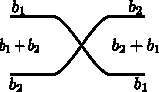
\includegraphics{diagrams/thesis/swap_plus.pdf}
\end{center}


\begin{center}
  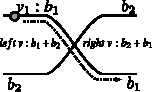
\includegraphics{diagrams/thesis/swap_plus_value.pdf}
\end{center}
  
\end{multicols}


\begin{small}
  \begin{multicols}{2}

    Thus

    {{~~~~~~ not : bool <--> bool }}

    {{~~~~~~ not = swap+}} 

    and we can verify that: 

    {{~~~~~~~~~~~~~~not true |--> false}}

    {{~~~~~~~~~~~~~~not false |--> true}}

    
  \end{multicols}
\end{small}

    \begin{itemize}
    \item Computation is modeled as the flow of particles in a
      circuit.

      \begin{itemize}
      \item Geometry of Interaction
      \item Proof Nets 
      \item Penrose diagrams for categories etc.
      \end{itemize}
    \end{itemize}
%\end{itemize}

\vfill

\end{frame}


%%%%%%%%%%%%%%%%%%%%%%%%%%%%%%%%%%%%%%%%%%%%%%%%%%%%%%%%%%%%%%%%%%%%%%%%%%
\begin{frame}{ {{langRevT}} examples : Conditionals}
  
% \vfill
\begin{itemize}

\item
{{ if_c (flag, b) = if (flag==true) then (flag, c(b)) else (flag, b) }}

\pause
\vfill

\begin{multicols}{2}
\begin{center}
  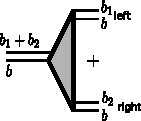
\includegraphics{diagrams/thesis/dist.pdf}
\end{center}


\begin{center}
  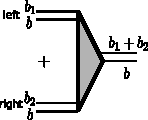
\includegraphics{diagrams/thesis/factor.pdf}
\end{center}
  
\end{multicols}

\pause
\vfill

\begin{multicols}{2}
\begin{center}
  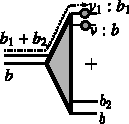
\includegraphics{diagrams/thesis/dist-wire-value1.pdf}
\end{center}


\begin{center}
  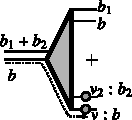
\includegraphics{diagrams/thesis/dist-wire-value2.pdf}
\end{center}
  
\end{multicols}


%% {{if_c : bool * b <--> bool * b }}

%% {{ if_c = dist (;) ((id (*) c) (+) id) (;) factor}}

% \pause
% \item {{cnot = if_{not} }} and {{toffoli = if_{cnot} }}
\end{itemize}

\end{frame}

%%%%%%%%%%%%%%%%%%%%%%%%%%%%%%%%%%%%%%%%%%%%%%%%%%%%%%%%%%%%%%%%%%%%%%%%%%
\begin{frame}{ {{langRevT}} examples : Conditionals}
  
% \vfill
\begin{itemize}

\item
{{ if_c (flag, b) = if (flag==true) then (flag, c(b)) else (flag, b) }}

\pause
\vfill

\item
{{if_c : bool * b <--> bool * b }}

{{ if_c = dist (;) ((id (*) c) (+) id) (;) factor}}

\vfill

\begin{center}
  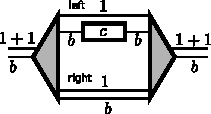
\includegraphics{diagrams/thesis/cnot.pdf}
\end{center}


\vfill
% \pause
% \item {{cnot = if_{not} }} and {{toffoli = if_{cnot} }}
\end{itemize}

\end{frame}



%%%%%%%%%%%%%%%%%%%%%%%%%%%%%%%%%%%%%%%%%%%%%%%%%%%%%%%%%%%%%%%%%%%%%%%%%%
\begin{frame}{ {{langRevT}} examples : Abstract Machines}

  \begin{multicols}{2}
    
%subcode{bnf} include main
% Numbers, n, m = 0 | n + 1
% Machine states = <n, n>

%subcode{bnf} include main
% Start state = <n, 0>
% Stop State = <0, n>
  \end{multicols}

%subcode{opsem} include main
% <n+1, m> |--> <n, m+1>

\vfill

\begin{center}
  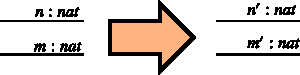
\includegraphics{iso-int/diagrams/nat-nat1.pdf}
\end{center}

\vfill

\end{frame}

%%%%%%%%%%%%%%%%%%%%%%%%%%%%%%%%%%%%%%%%%%%%%%%%%%%%%%%%%%%%%%%%%%%%%%%%%%
\begin{frame}{ {{langRevT}} examples : Abstract Machines}

  \begin{multicols}{2}
    
%subcode{bnf} include main
% Numbers, n, m = 0 | n + 1
% Machine states = <n, n>

%subcode{bnf} include main
% Start state = <n, 0>
% Stop State = <0, n>
  \end{multicols}

%subcode{opsem} include main
% <n+1, m> |--> <n, m+1>

\vfill

\begin{center}
  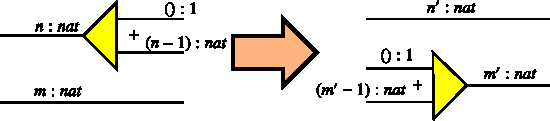
\includegraphics{iso-int/diagrams/nat-nat3.pdf}
\end{center}


\vfill
\begin{center}
  {{fold_{nat} : 1 + nat <--> nat  : unfold_{nat} }}

  {{nat = @@x.(1+x)}}
\end{center}
  
\vfill

\end{frame}

%%%%%%%%%%%%%%%%%%%%%%%%%%%%%%%%%%%%%%%%%%%%%%%%%%%%%%%%%%%%%%%%%%%%%%%%%%
\begin{frame}{ {{langRevT}} examples : Abstract Machines}

  \begin{multicols}{2}
    
%subcode{bnf} include main
% Numbers, n, m = 0 | n + 1
% Machine states = <n, n>

%subcode{bnf} include main
% Start state = <n, 0>
% Stop State = <0, n>
  \end{multicols}

%subcode{opsem} include main
% <n+1, m> |--> <n, m+1>

\vfill

\begin{center}
  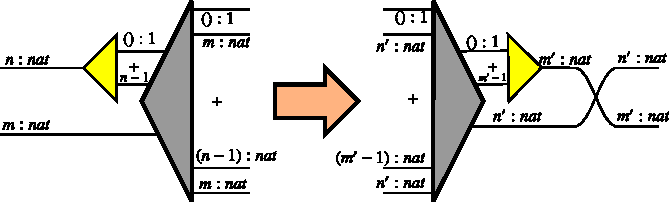
\includegraphics{iso-int/diagrams/nat-nat4.pdf}
\end{center}

  
\vfill

\end{frame}

%%%%%%%%%%%%%%%%%%%%%%%%%%%%%%%%%%%%%%%%%%%%%%%%%%%%%%%%%%%%%%%%%%%%%%%%%%
\begin{frame}{ {{langRevT}} examples : Abstract Machines}

  \begin{multicols}{2}
    
%subcode{bnf} include main
% Numbers, n, m = 0 | n + 1
% Machine states = <n, n>

%subcode{bnf} include main
% Start state = <n, 0>
% Stop State = <0, n>
  \end{multicols}

%subcode{opsem} include main
% <n+1, m> |--> <n, m+1>

\vfill

\begin{center}
  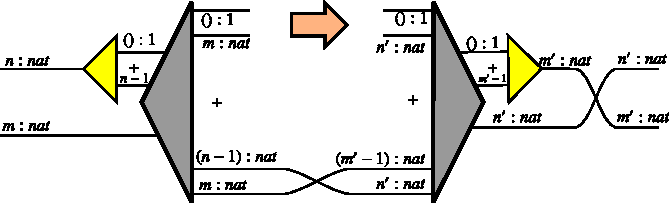
\includegraphics{iso-int/diagrams/nat-nat5.pdf}
\end{center}

  
\vfill

\end{frame}


%%%%%%%%%%%%%%%%%%%%%%%%%%%%%%%%%%%%%%%%%%%%%%%%%%%%%%%%%%%%%%%%%%%%%%%%%%
\begin{frame}{ {{langRevT}} examples : Abstract Machines}

  \begin{multicols}{2}
    
%subcode{bnf} include main
% Numbers, n, m = 0 | n + 1
% Machine states = <n, n>

%subcode{bnf} include main
% Start state = <n, 0>
% Stop State = <0, n>
  \end{multicols}

%subcode{opsem} include main
% <n+1, m> |--> <n, m+1>

\vfill

\begin{center}
  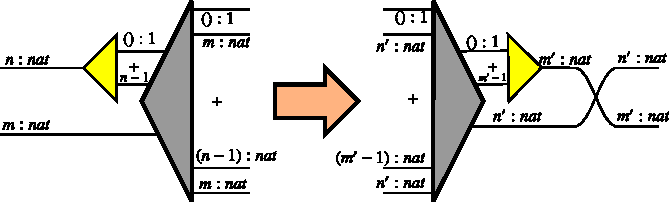
\includegraphics{iso-int/diagrams/nat-nat4.pdf}
\end{center}

  
\vfill

\end{frame}

%%%%%%%%%%%%%%%%%%%%%%%%%%%%%%%%%%%%%%%%%%%%%%%%%%%%%%%%%%%%%%%%%%%%%%%%%%
\begin{frame}{ {{langRevT}} examples : Abstract Machines}


\vfill

\begin{center}
\scalebox{0.6}{
  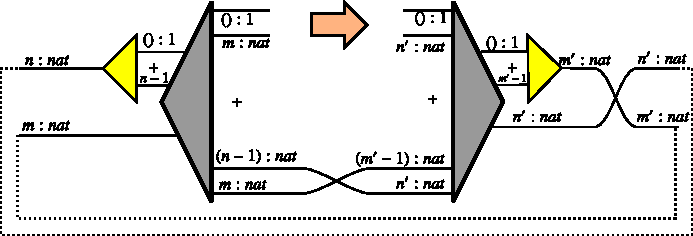
\includegraphics{iso-int/diagrams/nat-nat6.pdf}
}
\end{center}

\vfill

\begin{center}
\scalebox{0.6}{
  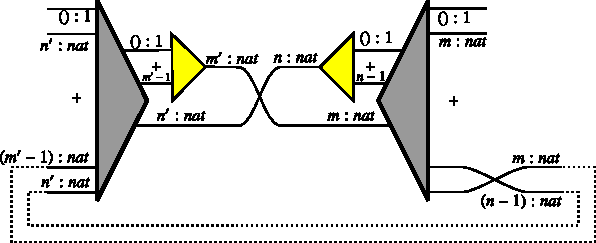
\includegraphics{iso-int/diagrams/nat-nat7.pdf}
}
\end{center}

\vfill

\end{frame}

%%%%%%%%%%%%%%%%%%%%%%%%%%%%%%%%%%%%%%%%%%%%%%%%%%%%%%%%%%%%%%%%%%%%%%%%%%
\begin{frame}{ {{langRevT}} examples : Abstract Machines}

  \begin{multicols}{2}
    
%subcode{bnf} include main
% Numbers, n, m = 0 | n + 1
% Machine states = <n, n>

%subcode{bnf} include main
% Start state = <n, 0>
% Stop State = <0, n>
  \end{multicols}

%subcode{opsem} include main
% <n+1, m> |--> <n, m+1>

\vfill

\begin{center}
  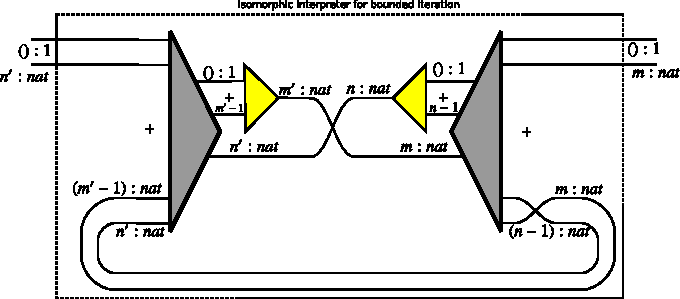
\includegraphics{iso-int/diagrams/nat-nat8.pdf}
\end{center}

  
\vfill

\end{frame}


%%%%%%%%%%%%%%%%%%%%%%%%%%%%%%%%%%%%%%%%%%%%%%%%%%%%%%%%%%%%%%%%%%%%%%%%%%
\begin{frame}{ {{langRevT}} examples : Metacircular Evaluator}

  \begin{scriptsize}
    
%subcode{bnf} include main
% Combinators, c = iso | c (;) c | c (*) c | c (+) c | trace c
% Combinator Contexts, cc = [] | Fst cc c | Snd c cc 
%                  &|& LeftTimes cc c v | RightTimes c v cc 
%                  &|& LeftPlus cc c | RightPlus c cc | Trace cc
% Values, v = () | (v, v) | L v | R v
%
% Machine states = <c, v, cc> | {[c, v, cc]}
% Start state = <c, v, []> 
% Stop State = {[c, v, []]}


%subcode{opsem} include main
%! columnStyle = rclr
% <iso, v, cc> &|-->& {[iso, iso(v), cc]} &~~~~~~~~~~~~ rule 1
% <c1(;)c2, v, cc> &|-->& <c1, v, Fst cc c2> &~~~~~~~~~~~~ rule 2
% {[c1, v, Fst cc c2]} &|-->& <c2, v, Snd c1 cc> &~~~~~~~~~~~~ rule 3
% {[c2, v, Snd c1 cc]} &|-->& {[ c1(;)c2, v, cc ]} &~~~~~~~~~~~~ rule 4
% <c1(+)c2, L v, cc> &|-->& <c1, v, LeftPlus cc c2> &~~~~~~~~~~~~ rule 5
% {[ c1, v, LeftPlus cc c2 ]} &|-->& {[c1 (+) c2, L v, cc ]} &~~~~~~~~~~~~ rule 6
% <c1(+)c2, R v, cc> &|-->& <c2, v, RightPlus c1 cc> &~~~~~~~~~~~~ rule 7
% {[ c2, v, RightPlus c1 cc ]} &|-->& {[c1 (+) c2, R v, cc ]} &~~~~~~~~~~~~ rule 8
% <c1(*)c2, (v1, v2), cc> &|-->& <c1, v1, LeftTimes cc c2 v2> &~~~~~~~~~~~~ rule 9
% {[ c1, v1, LeftTimes cc c2 v2 ]} &|-->& <c2, v2, RightTimes c1 v1 cc> &~~~~~~~~~~~~ rule 10
% {[ c2, v2, RightTimes c1 v1 cc ]} &|-->& {[ c1 (*) c2, (v1, v2), cc ]} &~~~~~~~~~~~~ rule 11
% < trace c, v, cc> &|-->& <c, R v, Trace cc> &~~~~~~~~~~~~ rule 12
% {[c, L v, Trace cc]} &|-->& <c, L v, Trace cc> &~~~~~~~~~~~~ rule 13
% {[c, R v, Trace cc]} &|-->& {[trace c, R v, cc]} &~~~~~~~~~~~~ rule 14

  \end{scriptsize}

\end{frame}


%%%%%%%%%%%%%%%%%%%%%%%%%%%%%%%%%%%%%%%%%%%%%%%%%%%%%%%%%%%%%%%%%%%%%%%%%%
\begin{frame}{ {{langRevT}} examples : Metacircular Evaluator}

\begin{center}
\scalebox{0.7}{
  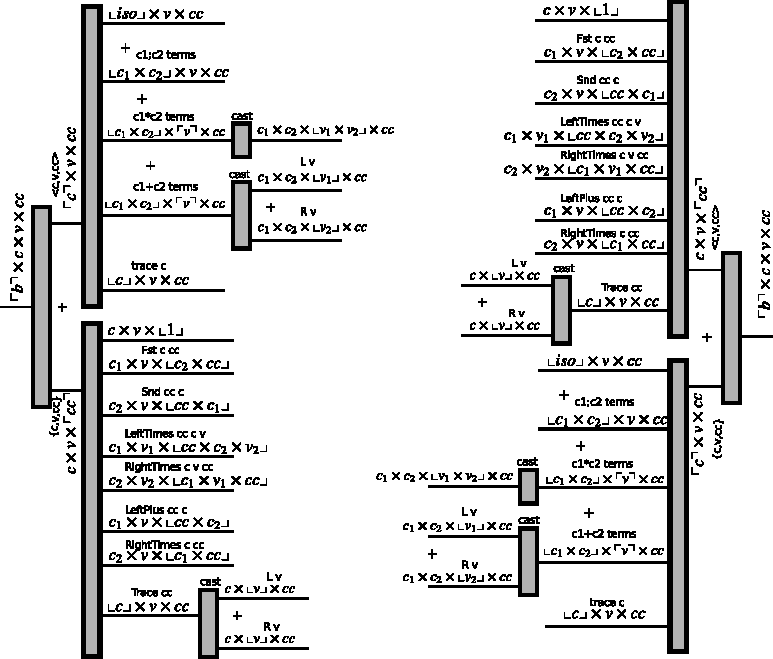
\includegraphics{iso-int/diagrams/pi0-1.pdf}
}
\end{center}

\end{frame}

%%%%%%%%%%%%%%%%%%%%%%%%%%%%%%%%%%%%%%%%%%%%%%%%%%%%%%%%%%%%%%%%%%%%%%%%%%
\begin{frame}{ {{langRevT}} examples : Metacircular Evaluator}


\begin{center}
\scalebox{0.7}{
  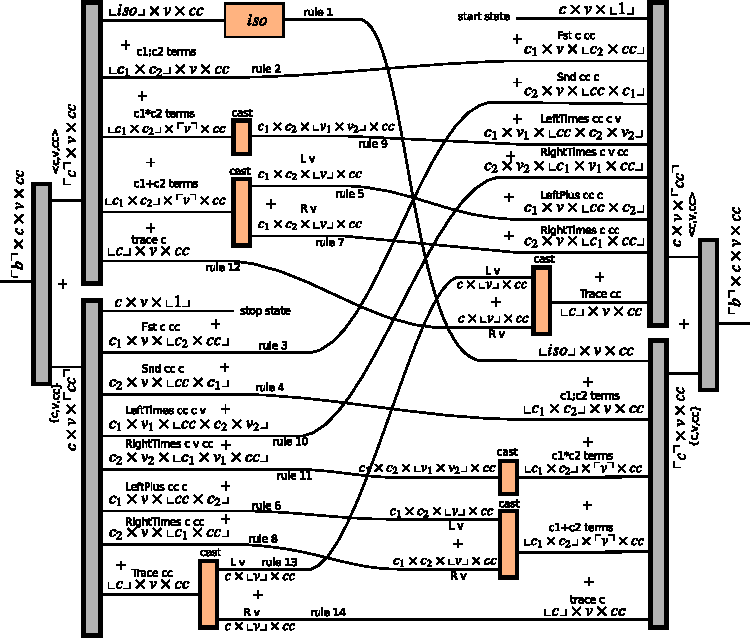
\includegraphics{iso-int/diagrams/pi0-2.pdf}
}
\end{center}

\end{frame}


%%%%%%%%%%%%%%%%%%%%%%%%%%%%%%%%%%%%%%%%%%%%%%%%%%%%%%%%%%%%%%%%%%%%%%%%%%%%
\begin{frame}
  
    \begin{center}
      \framebox{ Extending {{langRev}} with Information Effects }
    \end{center}


\end{frame}


%%%%%%%%%%%%%%%%%%%%%%%%%%%%%%%%%%%%%%%%%%%%%%%%%%%%%%%%%%%%%%%%%%%%%%%%%
\begin{frame}
\frametitle{Language of Information Effects : {{langArrT}} }

\vfill
%\begin{itemize}

\begin{block}

  Information effects are captured using an \red{arrow-metalanguage
    over {{langRevT}} } --- similar to expressing computational
  effects over \lcal using arrows or monads.
  
\end{block}

\vfill
\pause
\begin{enumerate}
\item {{langArrT}} extends {{langRevT}} with the arrow type \red{
    {{a:b1~~>b2}} }.

\vfill
\pause
\item Lifts traces, sequencing and parallel composition to the new
  arrow type {{b1 ~~> b2}}.


\vfill
\item And adds two information effects representing the creation and
  erasure of information.
  \begin{itemize}
  \item {{create : 1 ~~> b}}
  \item {{erase : b ~~> 1}}
  \end{itemize}

\vfill
  \item Given the ability to {{create}} constants, we can construct a
    {{clone}} operator.

\end{enumerate}


\vfill

\end{frame}




%%%%%%%%%%%%%%%%%%%%%%%%%%%%%%%%%%%%%%%%%%%%%%%%%%%%%%%%%%%%%%%%%%%%%%%%%%%%
\begin{frame}
  
    \begin{center}
      \framebox{ {{STLCfor ==> langArrT ==> langRevT}} }
    \end{center}


\end{frame}



%%%%%%%%%%%%%%%%%%%%%%%%%%%%%%%%%%%%%%%%%%%%%%%%%%%%%%%%%%%%%%%%%%%%%%%%%%%%
\begin{frame}{Translation 1: {{STLCfor ==> langArrT}} }
  
    \vfill

    \begin{block}

      We show the translation from a first-order {{STLC}}, with sum
      and product types, and extended with iteration to {{langArrT}}.

      \begin{center}
        {{ {@1@ G |- e : b ==> a : G^{*} ~~> b @} }}
      \end{center}
    \end{block}



  \begin{itemize}
    \vfill
  \item The translation exposes the implicit irreversibility of the
    \lcal by requiring explicit {{create}} and {{erase}} operations.

  \end{itemize}
  \vfill

\end{frame}


\begin{frame}{Translation 1 : overview}

  \begin{itemize}


\item Case {{let x = e1 in e2}}:
%subcode{proof} include main, trans1
%@ G |- e1 : b1 ==>  a1 : Gx ~~> b1
%@@! G, x : b1 |- e2 : b2 ==>  a2 : Gx * b1 ~~> b2
%@@@ G |- let x = e1 in e2 : b2  ==> a : Gx ~~> b2

%% To construct the required {{a}} we first clone {{Gx}}. We can apply~{{a1}}
%% to one of the copies to get {{b1}}.  The resulting value of type {{Gx*b1}}
%% is the input required by {{a2}} which returns the result of type {{b2}}:

\begin{center}
\scalebox{1.2}{
%subcode-line{pdfimage}[diagrams/let_binding.pdf]
}
\end{center}

  \end{itemize}

  
\end{frame}


%%%%%%%%%%%%%%%%%%%%%%%%%%%%%%%%%%%%%%%%%%%%%%%%%%%%%%%%%%%%%%%%%%%%%%%%%%%%
\begin{frame}{Translation 1 : overview}

\vfill
  \begin{itemize}


    \vfill
  \item The main work of the translation is to

  \begin{itemize}
  \item Make the implicit environment of {{STLCfor}} explicit as the {{G^*}} input.
  \item Thread the environment through the computation.
  \item Clone/introduce constants as required. 
  \item Erase unwanted values.
  \end{itemize}

\vfill
  \item Much of the complexity lies in the handling of sums and {{case}}. 

\vfill
  \item The product fragment of this translation is much like the
    {{CCC}} semantics for {{STLC}}.

  \end{itemize}
\vfill  

\end{frame}



%%%%%%%%%%%%%%%%%%%%%%%%%%%%%%%%%%%%%%%%%%%%%%%%%%%%%%%%%%%%%%%%%%%%%%%%%%%%
\begin{frame}{Translation 2: {{langArrT ==> langRevT}} }
  
    \vfill

    \begin{block}

      {{langArrT}} can be embedded in {{langRevT}}. 

    \begin{center}
      {{ {@1@ a : G^{*} ~~> b ==> c : h * G^* <--> g * b @} }}
    \end{center}

  \end{block}

  \begin{itemize}
\vfill
\item Information effects manifest as interactions with an information
  environment.

%% \item Irreversible {{langArrT}} programs with explicit information
%%   effects can be modeled by reversible {{langRevT}} programs where
%%   the information effects manifest as interactions with an information
%%   environment.

  \begin{itemize}
  \item The artifacts {{h}} and {{g}}, exposed in the types, represent
    this information environment.
  \end{itemize}

\end{itemize}
\vfill

\end{frame}


%%%%%%%%%%%%%%%%%%%%%%%%%%%%%%%%%%%%%%%%%%%%%%%%%%%%%%%%%%%%%%%%%%%%%%%%%%%%
\begin{frame}{Translation 2 : overview}

  \begin{itemize}


\item {{a1 >>> a2}}:
%subcode{proof} include main, trans1
%@ a1 : b1 ~~> b2 ==> c1 : h1 * b1 <--> g1 * b2 
%@@! a2 : b2 ~~> b3 ==> c2 : h2 * b2 <--> g2 * b3
%@@@ a1 >>> a2 : b1 ~~> b3 ==> c: h * b1 <--> g * b3

We choose {{h = h1 * h2}} and {{g = g1 * g2}} and we have 

\begin{center}
\scalebox{1.2}{
%subcode-line{pdfimage}[diagrams/seq_ggg.pdf]
}
\end{center}

  \end{itemize}

  
\end{frame}

%%%%%%%%%%%%%%%%%%%%%%%%%%%%%%%%%%%%%%%%%%%%%%%%%%%%%%%%%%%%%%%%%%%%%%%%%%%%
\begin{frame}{Translation 2 : overview}

\vfill
  \begin{itemize}


  \item The main work of the translation is to shuffle {{h}} and {{g}}
    values through the computation.

\vfill
  \item In the simplest sense, {{create}} exposes the input heap.

%subcode{proof} include main, trans1
%@ ~
%@@ create : 1 ~~> b ==> c: h * 1 <--> g * b

We choose {{h = b}} and {{g = 1}} and we have \red{ {{c = swap*}} }. 

\vfill
\item The operator {{erase}} does the dual and is also realized by
  {{swap*}}.


  \end{itemize}
\vfill  

  \begin{block}

    \begin{scriptsize}
      Note: The paper refines this further and gives two different
      treatments of {{create}}, one for {{langRevT}} and one for its
      strong-normalizing fragment {{langRev}}.
    \end{scriptsize}
  \end{block}


\end{frame}




% %%%%%%%%%%%%%%%%%%%%%%%%%%%%%%%%%%%%%%%%%%%%%%%%%%%%%%%%%%%%%%%%%%%%%%%%%
% \begin{frame}
% \frametitle{Non-termination and {{inc : nat <-> nat}} }

% \begin{itemize}
% \item {{ nat = @@x.1+x }}
% \item {{0 = <left ()>, 1 = <right 0>, 2 = <right 1>}}...
% \item {{fold : 1 + nat <-> nat : unfold}}
% \end{itemize}

% \vfill
% \begin{center}
% \scalebox{3.0}{
% %subcode-line{pdfimage}[../diagrams/inc_nat.pdf]
% }
% \end{center}

% \pause
% \vfill
% %subcode{opsem} include main
% %! columnStyle = rlrll
% % inc n &|--> (n+1) & ~~~~~~~inc^{-1}~ &(n+1) &|--> n
% % & & ~~~~~~~inc^{-1}~ &0 &|--> {@2@undefined@} 

% \begin{itemize}
% \item {{langRev}} can express infinite loops. 
% \end{itemize}

% \vfill
% \end{frame}


%%%%%%%%%%%%%%%%%%%%%%%%%%%%%%%%%%%%%%%%%%%%%%%%%%%%%%%%%%%%%%%%%%%%%%%%%%%%
\begin{frame}
  
    \begin{center}
      \framebox{ Entropy Analysis Example : {{langArrT}} }
    \end{center}


\end{frame}


\begin{frame}{XOR and NAND example : entropy analysis}
  
\vfill

  {{xor(b1, b2) = if b1 then (if b2 then false else true) else b2 }}

  {{nand(b1, b2) = if b1 then (if b2 then false else true) else true }}

\pause
\vfill

\begin{itemize}
\item Entropy of a function is {{ H_i - H_o }}
\item Entropy of input, {{H_i}}, for {{bool * bool}} is 2 bits. 

\pause
\item For {{xor}}, 
  \begin{itemize}
  \item Probability of output being true, {{P(true) = 1/2}}
  \item and {{P(false) = 1/2}}. 
  \item Therefore {{H_o = }} $-\sum p_i \log{p_i}$ {{ = 1}} bits. 
  \item Information lost is {{2 - 1 = 1 bit}}
  \end{itemize}
\pause

\item For {{nand}}, 
  \begin{itemize}
  \item Probability of output being true, {{P(true) = 3/4}}
  \item and {{P(false) = 1/4}}. 
  \item Therefore {{H_o = }} $-\sum p_i \log{p_i} = 1/4 \log{4} + 3/4
    (\log{4}-\log{3}) = 0.8$ bits.
  \item Information lost is {{2 - 0.8 = 1.2 bits}}
  \end{itemize}

\end{itemize}

\vfill


\end{frame}


%%%%%%%%%%%%%%%%%%%%%%%%%%%%%%%%%%%%%%%%%%%%%%%%%%%%%%%%%%%%%%%%%%%%%%%%%%%%%%%
\begin{frame}{XOR and NAND example : {{langArrT}} implementation}
  
\vfill

\begin{itemize}

\item The most optimal implementation of {{xor}} must erase at least 1
  bit i.e. there must be at least one {{erase_{bool} }}.

  \begin{block}
    


{{ xor : bool * bool ~~> bool }}

{{ xor = dist >>> (not +++ id) }} 

{{~~~~~~~~ >>> factor >>> (erase_{bool} *** id) >>> arr identl*}}

  \end{block}

\vfill

\item The most optimal implementation of {{nand}} must erase at least
  1.2 bits i.e. at least two {{bools}} must be erased. 


  \begin{block}
    
{{ nand : bool * bool ~~> bool }}

{{ nand = dist >>> (not +++ (erase_{bool} >>> create_{true})) }} 

{{~~~~~~~ >>> factor >>> (erase_{bool} *** id) >>> arr identl* }}

  \end{block}

\vfill

\item These minimums are captured in the structure of the program.


\end{itemize}





\vfill

\end{frame}


%%%%%%%%%%%%%%%%%%%%%%%%%%%%%%%%%%%%%%%%%%%%%%%%%%%%%%%%%%%%%%%%%%%%%%%%%
\begin{frame}
\frametitle{Applications and Connections}

\begin{itemize}

\vfill
\item Could serve as better basis of computation than \lcal for
  applications where information manipulation is computationally
  significant.

  \begin{itemize}
  \item Quantitative information-flow security.~\cite{myerssab}
  \item Differential privacy.~\cite{dwork:differential}
  \item Energy-aware computing.~\cite{1324180,605411}
  \item VLSI design.~\cite{Macii:1996:ECE:874066.875828}
  \item Biochemical models of computation.~\cite{bio}

  \end{itemize}

\vfill

\item Hiding in the structure of {{langRevT}} is a Dagger Symmetric
  Traced Monoidal Category.

  \begin{itemize}
  \item GoI. \cite{girard1989geometry}

  \item Duality of Computation. \cite{Filinski:1989:DCI:648332.755574}, \cite{curien00duality}.

  \item Quantum Computing. 

  \item Categorical constructions such as \ensuremath{\mathcal{G}} and \textbf{Int}. 

  \end{itemize}

\end{itemize}

\vfill

\end{frame}


%%%%%%%%%%%%%%%%%%%%%%%%%%%%%%%%%%%%%%%%%%%%%%%%%%%%%%%%%%%%%%%%%%%%%%%%%
%%%%%%%%%%%%%%%%%%%%%%%%%%%%%%%%%%%%%%%%%%%%%%%%%%%%%%%%%%%%%%%%%%%%%%%%%
\begin{frame}

\vfill
  \begin{center}
    \framebox{
    The Dualities of Computation}
  \end{center}
\vfill

\end{frame}


%%%%%%%%%%%%%%%%%%%%%%%%%%%%%%%%%%%%%%%%%%%%%%%%%%%%%%%%%%%%%%%%%%%%%%%%%
\begin{frame}
\frametitle{Extensions: Duality}

\begin{itemize}
\vfill
\item How do we express functions in {{langRevT}}?

\vfill
\item How do we express continuations in {{langRevT}}?

\vfill
\end{itemize}


\end{frame}


%%%%%%%%%%%%%%%%%%%%%%%%%%%%%%%%%%%%%%%%%%%%%%%%%%%%%%%%%%%%%%%%%%%%%%%%%
\begin{frame}
\frametitle{Extensions: Duality}

Not one duality, but two: negative and fractional types. 

%subcode{opsem} include main
% eta+ &: 0 <-> (-b) + b :& eps+
% eta* &: 1 <-> (1/b) * b :& eps*

%subcode{proof} include main
%@ |- v : b
%@@ |- -v : -b
%
%@ |- v : b
%@@ |- 1/v : 1/b

\begin{multicols}{2}
\begin{center}
  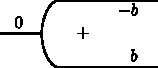
\includegraphics{diagrams/eta.pdf}
\end{center}
  
\begin{center}
 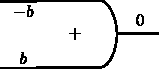
\includegraphics{diagrams/eps.pdf}
\end{center}
\end{multicols}
\begin{multicols}{2}
\begin{center}
  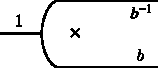
\includegraphics{diagrams/eta_times.pdf}
\end{center}
  
\begin{center}
  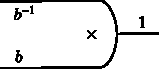
\includegraphics{diagrams/eps_times.pdf}
\end{center}
\end{multicols}


\end{frame}

%%%%%%%%%%%%%%%%%%%%%%%%%%%%%%%%%%%%%%%%%%%%%%%%%%%%%%%%%%%%%%%%%%%%%%%%%
\begin{frame}
\frametitle{Extensions: {{langRevEE}} }



\begin{multicols}{2}
\begin{center}
\scalebox{1.5}{
  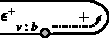
\includegraphics{diagrams/eps_plus1.pdf}
}
\end{center}
  
\begin{center}
\scalebox{1.5}{
  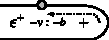
\includegraphics{diagrams/eps_plus2.pdf}
}
\end{center}  
\end{multicols}

\begin{center}
 Backward Information Flow. 
\end{center}

\begin{multicols}{2}
\begin{center}
\scalebox{1.5}{
  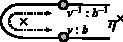
\includegraphics{diagrams/eta_times1.pdf}
}
\end{center}

\begin{center}
\scalebox{1.5}{
  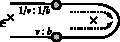
\includegraphics{diagrams/eps_times1.pdf}
}
\end{center}  
\end{multicols}

\begin{center}
 Creation and Annihilation of entangled particles. 
\end{center}


In many ways, we are only begining to understand these structures. 


\end{frame}




%%%%%%%%%%%%%%%%%%%%%%%%%%%%%%%%%%%%%%%%%%%%%%%%%%%%%%%%%%%%%%%%%%%%%%%%%
%%%%%%%%%%%%%%%%%%%%%%%%%%%%%%%%%%%%%%%%%%%%%%%%%%%%%%%%%%%%%%%%%%%%%%%%%
\begin{frame}

\vfill
  \begin{center}
    Extras
  \end{center}
\vfill

\end{frame}



% %%%%%%%%%%%%%%%%%%%%%%%%%%%%%%%%%%%%%%%%%%%%%%%%%%%%%%%%%%%%%%%%%%%%%%%%%
\begin{frame}
\frametitle{ The language {{langRevT}} }

% A programming language emerges:

\begin{block}{Syntax of {{langRevT}} }
%subcode{bnf} include main 
% base types, b ::= 0 | 1 | b+b | b*b {@1@ | x | @@x.b @}
% combinator types, t ::= b <--> b
% values, v ::= () | left v | right v | (v,v) {@1@ | <v> @}
%
% isomorphisms, iso ::= swap+ | assocl+ | assocr+ 
%                   &|& swap* | assocl* | assocr* | identl* | identr* 
%                   &|& dist | factor | id {@1@ | fold | unfold @}
% combinators, c ::= iso | sym c | c (;) c | c (*) c | c (+) c {@1@ | trace c @}

% base types, b ::= 0 | 1 | b+b | b*b {@1@ | x | @@x.b @}
% values, v ::= () | left v | right v | (v,v) {@1@ | <v> @}
%
% isomorphisms, iso ::= swap+ | assocl+ | assocr+ | identl+ | identr+  
%                   &|& swap* | assocl* | assocr* | identl* | identr* 
%                   &|& dist0 | factor0 | dist | factor | id {@1@ | fold | unfold @}
% combinators, c ::= iso | sym c | c (;) c | c (*) c | c (+) c {@1@ | trace c @}
\end{block}

\begin{itemize}
\item {{langRev}} is the fragment of {{langRevT}} sans recursive types and trace. 
  \begin{itemize}
  \item i.e. without the red parts. 
  \end{itemize}
\end{itemize}


% \begin{itemize}

% \item {{langRev}} is a dagger symmetric monoidal category with a trace
%   over the monoid {{(+, 0)}}.

% \item In practice, we use ``wiring diagrams'' to program : values are
%   like particles moving through a circuit.

% \end{itemize}

% Draw ``wiring diagrams'' for programs. 

\end{frame}


% %%%%%%%%%%%%%%%%%%%%%%%%%%%%%%%%%%%%%%%%%%%%%%%%%%%%%%%%%%%%%%%%%%%%%%%%%
\begin{frame}{Logically reversible functions are ``information
    preserving''}

\vfill

  \begin{enumerate}


  \item \red{Logical reversibility}: A function $f : b_1 \rightarrow b_2$ is
    logically reversible if there exists an inverse function $g : b_2
    \rightarrow b_1$ such that for all values $v_1 \in b_1$ and $v_2
    \in b_2$, we have: $f(v_1) = v_2$ iff $g(v_2) =
    v_1$. (\cite{Zuliani:2001:LR})

  \item \red{Entropy of a variable} : Let `$b$' be a (not necessarily
    finite) type whose values are labeled $b^1, b^2, \ldots$. Let
    $\xi$ be a random variable of type $b$ that is equal to $b^i$ with
    probability $p_i$. The entropy of $\xi$ is defined as $-\sum p_i
    \log{p_i}$.

  \item \red{Output entropy of a function}: Consider a function
    {{f:b1->b2}} where {{b2}} is a (not necessarily finite) type whose
    values are labeled $b_2^1, b_2^2, \ldots$. The output entropy of
    the function is given by $- \sum q_j \log{q_j}$ where $q_j$
    indicates the probability of the output of the function to have
    value ${b_2}^j$.


  \item \red{Information Preservation}: We say a function is
    \emph{information-preserving} if its output entropy is equal to
    the entropy of its input.

  \item \red{Non-termination is not an observable}.

  \end{enumerate}

\vfill
  
\end{frame}


%%%%%%%%%%%%%%%%%%%%%%%%%%%%%%%%%%%%%%%%%%%%%%%%%%%%%%%%%%%%%%%%%%%%%%%%

\begin{frame} {We extend Toffoli's result in several ways}

  \begin{itemize}

 \vfill
  \item Richer types, not truth tables. (Full sum and product types)

    \vfill
  \item Term language for reversible and irreversible computation.

    \vfill
  \item Type directed translation.

    \vfill
  \item Deal with infinite functions (ex. over nats).
  \end{itemize}
\end{frame}



%% \begin{frame}
%% \frametitle{References}
%% \begin{scriptsize}



\begin{frame}
\frametitle{References}
\begin{scriptsize}

\bibliographystyle{plainnat}
\bibliography{cites}
\end{scriptsize}
\end{frame}


%% \end{scriptsize}
%% \end{frame}

\end{document}
